%%%%%%%%%%%%%%%%%%%%%%%%%%%%%%%%%%%%%%%%%
% University/School Laboratory Report
% LaTeX Template
% Version 3.1 (25/3/14)
%
% This template has been downloaded from:
% http://www.LaTeXTemplates.com
%
% Original author:
% Linux and Unix Users Group at Virginia Tech Wiki 
% (https://vtluug.org/wiki/Example_LaTeX_chem_lab_report)
%
% License:
% CC BY-NC-SA 3.0 (http://creativecommons.org/licenses/by-nc-sa/3.0/)
%
%%%%%%%%%%%%%%%%%%%%%%%%%%%%%%%%%%%%%%%%%

%----------------------------------------------------------------------------------------
%	PACKAGES AND DOCUMENT CONFIGURATIONS
%----------------------------------------------------------------------------------------

\documentclass[12pt]{article}

\usepackage{siunitx} % Provides the \SI{}{} and \si{} command for typesetting SI units
\usepackage{graphicx} % Required for the inclusion of images
\usepackage{natbib} % Required to change bibliography style to APA
\usepackage{amsmath} % Required for some math elements 
\usepackage[french]{babel}
\usepackage[utf8]{inputenc}
\usepackage[T1]{fontenc}

\usepackage{color}
\usepackage[top=1in, bottom=1.25in, left=1.25in, right=1.25in]{geometry}

\renewcommand{\labelenumi}{\alph{enumi}.} % Make numbering in the enumerate environment by letter rather than number (e.g. section 6)

%\usepackage{times} % Uncomment to use the Times New Roman font

%----------------------------------------------------------------------------------------
%	DOCUMENT INFORMATION
%----------------------------------------------------------------------------------------

\title{Décision de finales d'échecs\\ Comparaison d'implémentations \\ HPC} % Title

\author{Mathis \textsc{Caristan} \& Alexandre \textsc{Fernandez}} % Author name

\date{\today} % Date for the report

\begin{document}

\maketitle % Insert the title, author and date

\begin{abstract}
    Ce rapport présente la démarche suivie pour paralléliser un code de solveur d'échecs.
    Trois types d'implémentations ont été réalisées.
    Une purement MPI (avec la bilbiothèque OpenMPI), une deuxième purement OpenMP,
    et une troisième utilisant un mélange des deux.
    Le travail a été découpé en deux blocs distincts, tout d'abord la paralélisation
    du code \og naïf\fg. Puis L'extension de la paralélisation à une approche plus
    intelligente du problème qui utilise \og l'élagage alpha-bêta\fg.
    Les trois implémentations ont été réalisées pour les deux blocs, et les résultats
    sont comparés ici.
\end{abstract}

%----------------------------------------------------------------------------------------
%	SECTION 1
%----------------------------------------------------------------------------------------

\section{Introduction}
Nous considérons ici une version simplifiée du jeu d'échecs, dans laquelle on n'utilise
que les pions et rois. Nous nous sommes vus fournir le code séquentiel du solveur.
Celui-ci présentait deux paramètres d'optimisations, dont l'activation rendait le code
plus dur à paralléliser. Le premier était l'utilisation de l'algorithme négamax avec un
arbre alpha-bêta, et le second l'utilisation d'une table de transposition. Nous n'avons
pas traité le second paramètre d'optimisation. Le programme prend en entrée un état du
plateau en notation Fosryth-Edwards. Il cherche ensuite tous les coups possibles jusqu'à
un nombre de coups donné. Il joue tous les coups, et analyse quel est le meilleur choix
possible pour chaque joueur à chaque coups. Si il ne parvient pas à trouver une fin à la
partie, il réitère en jouant un coup supplémentaire jusqu'à trouver une issue à la partie.
\par Les performances du programme séquentiel sont données dans la table \ref{tab:seq}.
Ces valeurs serviront d'étalon pour mesurer les performances des parallélisations.
\begin{table} \begin{center}
    \begin{tabular}{|c|c|c||c|}
    \hline 
    \textbf{Optimisation}  & \textbf{Machine(s)}        & \textbf{Entrée}   & \textbf{Temps}\\ \hline
    \og Naïf \fg    &   gpu-3                           &   "7K//k1P/7p b"          &   ???\\ \hline
    \og Naïf \fg    &   14-15-401-05 à 14-15-401-12     &   "7K//k1P/7p b"          &   ???\\ \hline
    Alpha-bêta      &   gpu-3                           &   "/5p/4p/4P/4KP///k w"   &   ???\\ \hline
    Alpha-bêta      &   14-15-401-05 à 14-15-401-12     &   "/5p/4p/4P/4KP///k w"   &   ???\\ \hline
    \end{tabular} 
    \caption{\label{tab:seq}Temps d'éxecution du programme séquentiel pour différents paramètres.}
\end{center} \end{table}
\'Etant donné les temps d'exécution de ces instances, les temps d'exécution n'ont été mesurés
qu'une seule fois, et en conséquence, sont sujets à une incertitude de mesure liée à
la possible utilisation des machines par d'autre utilisateurs pendant la mesure.
Néanmoins, on observe qu'ils semblent en accord avec les valeurs prévues dans les les 
fichiers \texttt{positions\_v1.txt} et \texttt{positions\_v2.txt}.


\section{Parallélisation du code naïf}
    \subsection{MPI}
    Pour cette implémentation, nous avons fait le choix d'utiliser une 
    répartition de charge dynamique avec un modèle maître-esclave.
    Afin de ne pas subir un potentiel déséquilibre entre les différentes
    tâches, le maître prépare environ 10 fois plus de tâches qu'il n'y a
    de processus esclaves. Pour cela, il effectue un parcours en largeur
    jusqu'à arriver à une profondeur dont le nombre de branches vérifie le
    critère précédent. Nous nous appuyons sur une structure C, permettant de
    "remonter l'arbre" d'un noeud vers ses parents. La structure permet
    également d'accéder aux structures \texttt{tree\_t} et \texttt{result\_t}
    d'un noeud, pré-existante dans le code séquentiel.
    Ainsi, avec un tableau de cette structure que nous avons créée, le 
    processus maître maintient une liste des noeuds du haut de l'arbre,
    qu'il utilise ensuite pour distribuer le travail aux processus esclaves.\\
    \par Une fois que le maître a trouvé suffisemment de tâches, commence la
    répartition des tâches. Il envoie à chacun des processus esclaves, un
    couple de structures \texttt{tree\_t/result\_t} pour que celui-ci puisse
    appeler \texttt{evaluate}. Une fois sa tâche finie, un processus esclave 
    renvoie son résultat au processus 0, qui a son tour lui renvoie une
    nouvelle tâche à effectuer. Lorsqu'il n'y a plus de tâches à une profondeur
    donnée, les esclaves se bloquent et se mettent en attente. Le maître
    recombine alors les données des esclaves. Ce déroulement est illustré par
    la figure \ref{fig:time}. Lorsque le processus maître a identifié une
    situation correspondant à la fin de la partie, il indique aux esclaves
    qu'ils peuvent se terminer, avant de terminer lui-même.
    \begin{figure} \begin{center}
        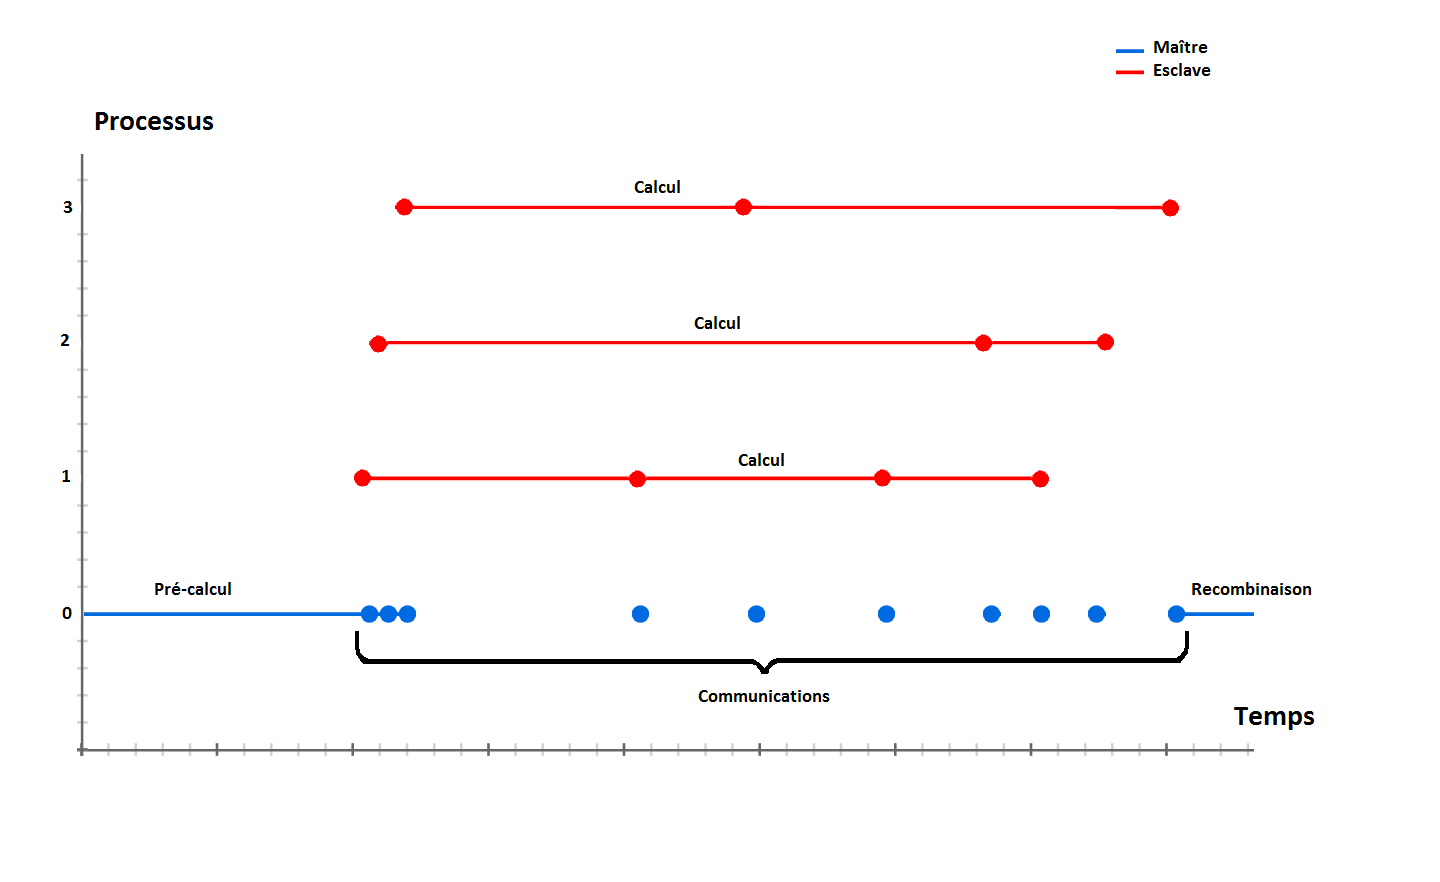
\includegraphics[scale=0.33]{figures/time}
        \caption{\label{fig:time}Illustration du fonctionnement du programme
        avec 4 processus. Le maître pré-calcul les tâches a distribuer,
        puis les communique aux esclaves. Les esclaves travaillent sur les
        tâches qui leurs sont attribuées avant de les renvoyer au maître.
        Enfin, le maître recombine les résultats ensemble.}
    \end{center} \end{figure}
    On note que le processus maître ne travaille pas pendant que les esclaves
    calculent.\\
    \par {\color{red} Ajouter les résultats (+ parler meta struct?
    + avancée par rapport à la premiere deadline?)}
    \subsection{OMP}
    \subsection{OMP + MPI}
    Cette implémentation reprend simplement 
    les principes des deux premières. Un processus maître prépare des tâches
    qui sont ensuite distribuées aux esclaves. Ceux-ci utilisent alors OpenMP
    pour paralléliser le calcul de leur tâche, avant de renvoyer le résultat
    au maître.\\
    \par {\color{red} Ajouter les résultats}
    \subsection{Analyse et comparaison}

\section{Parallélisation avec alpha-bêta}
    \subsection{MPI}
    L'approche alpha-bêta propose d'élaguer les branches
    les moins intéressantes au fur et à mesure de la progression de 
    l'algorithme. De plus, une fonction nous permet de trier les coups
    possibles du plus au moins intéressant. Dès lors, une nouvelle 
    approche semblait pertinente ; nous avons choisi de faire jouer au
    maître toute la branche la plus à gauche de l'arbre, soit
    probablement les meilleurs coups (d'après une heuristique qui n'est pas 
    exacte). Il élague ensuite les branches en fonction de ce premier
    parcours. Ensuite, nous appliquons à nouveau le principe utilisé pour
    la version naïve. Le maître génère un nombre de tâches suffisamment
    important puis les distribue aux esclaves. Une différence existe
    néanmoins avec la version précédente, lorsqu'il reçoit des résultats,
    il les analyse immédiatement, afin d'effectuer les coupes nécessaires
    si besoin. Dans la version naïve, l'analyse des résultats était
    effectuée collectivement une fois tous les résultats obtenus.
    Notons également l'introduction d'un paramètre supplémentaire pour
    la quantité de tâches générées. En effet, nous demandons que le maître
    génère $k*nb_{proc}$ tâches. Nous avons fait des essais avec plusieurs
    valeurs de $k$. Cette idée nous est venue en considérant que les coupes
    allaient probablement diminuer le nombre de tâches à effectivement
    analyser par les esclaves, augmentant la possibilité de déséquilibre
    de charge. Les résultats obtenus sont présentés dans la table
    \ref{tab:alpha}
    \begin{table} \begin{center}
    	\begin{tabular}{|c|c|c|}
    	\hline
    	??? & ??? & ??? \\ \hline
    	\end{tabular}
    	\caption{\label{tab:alpha}\color{red} résultats}
    \end{center} \end{table}
    \subsection{OMP}
    \subsection{OMP + MPI}
    \subsection{Résultats et analyse}

% ------------------------------------------
%           Début du template
% ------------------------------------------
%%%   \section{Objective}
%%%   
%%%   To determine the atomic weight of magnesium via its reaction with oxygen and to study the stoichiometry of the reaction (as defined in \ref{definitions}):
%%%   
%%%   \begin{center}$E = mc^2$\end{center}
%%%   
%%%   % If you have more than one objective, uncomment the below:
%%%   %\begin{description}
%%%   %\item[First Objective] \hfill \\
%%%   %Objective 1 text
%%%   %\item[Second Objective] \hfill \\
%%%   %Objective 2 text
%%%   %\end{description}
%%%   
%%%   \subsection{Definitions}
%%%   \label{definitions}
%%%   \begin{description}
%%%   \item[Stoichiometry]
%%%   The relationship between the relative quantities of substances taking part in a reaction or forming a compound, typically a ratio of whole integers.
%%%   \item[Atomic mass]
%%%   The mass of an atom of a chemical element expressed in atomic mass units. It is approximately equivalent to the number of protons and neutrons in the atom (the mass number) or to the average number allowing for the relative abundances of different isotopes. 
%%%   \end{description} 
%%%    
%%%   %----------------------------------------------------------------------------------------
%%%   %	SECTION 2
%%%   %----------------------------------------------------------------------------------------
%%%   
%%%   \section{Experimental Data}
%%%   
%%%   \begin{tabular}{ll}
%%%   Mass of empty crucible & \SI{7.28}{\gram}\\
%%%   Mass of crucible and magnesium before heating & \SI{8.59}{\gram}\\
%%%   Mass of crucible and magnesium oxide after heating & \SI{9.46}{\gram}\\
%%%   Balance used & \#4\\
%%%   Magnesium from sample bottle & \#1
%%%   \end{tabular}
%%%   
%%%   %----------------------------------------------------------------------------------------
%%%   %	SECTION 3
%%%   %----------------------------------------------------------------------------------------
%%%   
%%%   \section{Sample Calculation}
%%%   
%%%   \begin{tabular}{ll}
%%%   Mass of magnesium metal & = \SI{8.59}{\gram} - \SI{7.28}{\gram}\\
%%%   & = \SI{1.31}{\gram}\\
%%%   Mass of magnesium oxide & = \SI{9.46}{\gram} - \SI{7.28}{\gram}\\
%%%   & = \SI{2.18}{\gram}\\
%%%   Mass of oxygen & = \SI{2.18}{\gram} - \SI{1.31}{\gram}\\
%%%   & = \SI{0.87}{\gram}
%%%   \end{tabular}
%%%   
%%%   Because of this reaction, the required ratio is the atomic weight of magnesium: \SI{16.00}{\gram} of oxygen as experimental mass of Mg: experimental mass of oxygen or $\frac{x}{1.31}=\frac{16}{0.87}$ from which, $M_{E=mc^2} = 16.00 \times \frac{1.31}{0.87} = 24.1 = \SI{24}{\gram\per\mole}$ (to two significant figures).
%%%   
%%%   %----------------------------------------------------------------------------------------
%%%   %	SECTION 4
%%%   %----------------------------------------------------------------------------------------
%%%   
%%%   \section{Results and Conclusions}
%%%   
%%%   The atomic weight of magnesium is concluded to be \SI{24}{\gram\per\mol}, as determined by the stoichiometry of its chemical combination with oxygen. This result is in agreement with the accepted value.
%%%   
%%%   \begin{figure}[h]
%%%   \begin{center}
%%%   
\includegraphics[width=0.65\textwidth]{figures/placeholder} % Include the image placeholder.png
%%%   \caption{Figure caption.}
%%%   \end{center}
%%%   \end{figure}
%%%   
%%%   %----------------------------------------------------------------------------------------
%%%   %	SECTION 5
%%%   %----------------------------------------------------------------------------------------
%%%   
%%%   \section{Discussion of Experimental Uncertainty}
%%%   
%%%   The accepted value (periodic table) is \SI{24.3}{\gram\per\mole} \cite{Smith:2012qr}. The percentage discrepancy between the accepted value and the result obtained here is 1.3\%. Because only a single measurement was made, it is not possible to calculate an estimated standard deviation.
%%%   
%%%   The most obvious source of experimental uncertainty is the limited precision of the balance. Other potential sources of experimental uncertainty are: the reaction might not be complete; if not enough time was allowed for total oxidation, less than complete oxidation of the magnesium might have, in part, reacted with nitrogen in the air (incorrect reaction); the magnesium oxide might have absorbed water from the air, and thus weigh ``too much." Because the result obtained is close to the accepted value it is possible that some of these experimental uncertainties have fortuitously cancelled one another.
%%%   
%%%   %----------------------------------------------------------------------------------------
%%%   %	SECTION 6
%%%   %----------------------------------------------------------------------------------------
%%%   
%%%   \section{Answers to Definitions}
%%%   
%%%   \begin{enumerate}
%%%   \begin{item}
%%%   The \emph{atomic weight of an element} is the relative weight of one of its atoms compared to C-12 with a weight of 12.0000000$\ldots$, hydrogen with a weight of 1.008, to oxygen with a weight of 16.00. Atomic weight is also the average weight of all the atoms of that element as they occur in nature.
%%%   \end{item}
%%%   \begin{item}
%%%   The \emph{units of atomic weight} are two-fold, with an identical numerical value. They are g/mole of atoms (or just g/mol) or amu/atom.
%%%   \end{item}
%%%   \begin{item}
%%%   \emph{Percentage discrepancy} between an accepted (literature) value and an experimental value is
%%%   \begin{equation*}
%%%   \frac{\mathrm{experimental\;result} - \mathrm{accepted\;result}}{\mathrm{accepted\;result}}
%%%   \end{equation*}
%%%   \end{item}
%%%   \end{enumerate}

%----------------------------------------------------------------------------------------
%	BIBLIOGRAPHY
%----------------------------------------------------------------------------------------

\bibliographystyle{apalike}

\bibliography{sample}

%----------------------------------------------------------------------------------------


\end{document}
